\documentclass{beamer}
%\documentclass{powerdot}
%\documentclass{slides}[14pt]
%\pagestyle{empty}
%\normalsize
\usepackage{amsmath}
\usepackage{amssymb}
\usepackage{amscd}
% \usepackage{moreverb}
\usepackage{graphicx}
% \usepackage[all]{xy}
% \usepackage{beamerthemesplit}


\input macros			   %% loan from John Gibson's snowbird 07 talk
% \input ../../inputs/defsThesis     %% all Vaggelis edits: \renewcommand, etc

% Setup appearance:

\usetheme{Darmstadt}
\usefonttheme[onlylarge]{structurebold}
\setbeamerfont*{frametitle}{size=\normalsize,series=\bfseries}
\setbeamertemplate{navigation symbols}{}


% Standard packages

\usepackage[english]{babel}
\usepackage[latin1]{inputenc}
\usepackage{times}
\usepackage[T1]{fontenc}


% % Setup TikZ
% 
% \usepackage{tikz}
% \usetikzlibrary{arrows}
% \tikzstyle{block}=[draw opacity=0.7,line width=1.4cm]

\title{Recurrent spatio-temporal structures in presence of continuous symmetries}
\author{Evangelos Siminos}
\institute{Center for Nonlinear Science\\ School of Physics\\ Georgia Institute of Technology}
\date{March 23, 2009}

\begin{document}

\begin{frame}
  \titlepage
\end{frame}

\begin{frame}{Outline}
  \tableofcontents
\end{frame}

\section{Introduction}

\subsection{Dynamicist's vision of Turbulence}

\begin{frame}{Turbulence}
 	
\end{frame}

\begin{frame}{PO's and beyond}
\end{frame}

\subsection{This thesis}

\begin{frame}{Symmetry}
\end{frame}

\begin{frame}{\KSe}
 
\end{frame}

\section{(De-)symmetrization}

\subsection{$G$-background}

\begin{frame}{Symmetry}

\begin{columns}
 \column{0.6\textwidth}
	\begin{itemize}
		\item A set has a symmetry if it is invariant under a transformation.
		\item Symmetry transformations form groups acting on \Rls{n}.
		\item Here we consider subgroups of \On{n}.
	\end{itemize}
 \column{0.3\textwidth}
	\begin{exampleblock}{Equilateral triangle}
	 	\begin{center}
			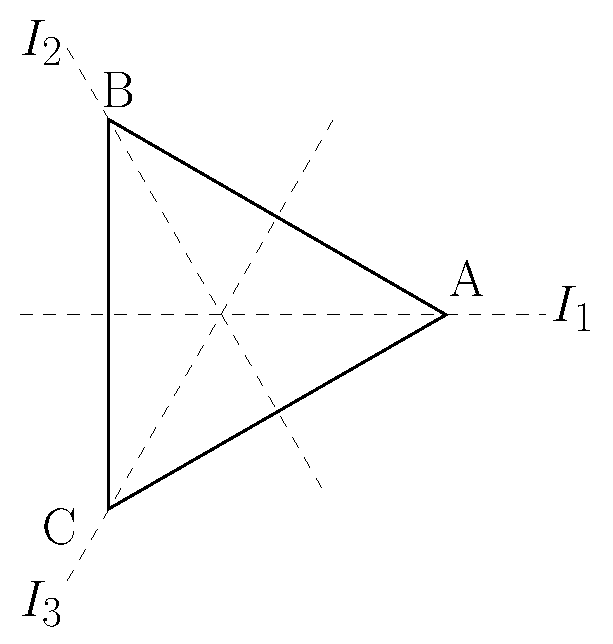
\includegraphics[width=.7\textwidth]{../../figs/D3triangle}
		\end{center}
	\Dn{3} acting on \Clx{} by
	\[
	\begin{split}	
  		\Drot z &= e^{i\frac{2\pi}{3}} z\,,\\
  		\Refl z  &= \conj{z}\,.
 	\end{split}
	\]
	\end{exampleblock}
\end{columns}

\end{frame}

\begin{frame}{Isotropy subgroups}

Not all points have the same symmetry:
\begin{columns}
  \column{0.7\textwidth}
	\begin{block}{Group orbit of $x$}
	\[
	\Gamma x = \{\gamma x: \gamma\in\Gamma\}\,.
	\]
	\end{block}
 	\begin{block}{Isotropy subgroup}
 	\[
 	\stab{x}=\{\gamma\in\Gamma:\gamma x=x\}\,.
 	\]
 	\end{block}
  \column{0.3\textwidth}
 	\begin{exampleblock}{Equilateral triangle}
 	 	\begin{center}
 			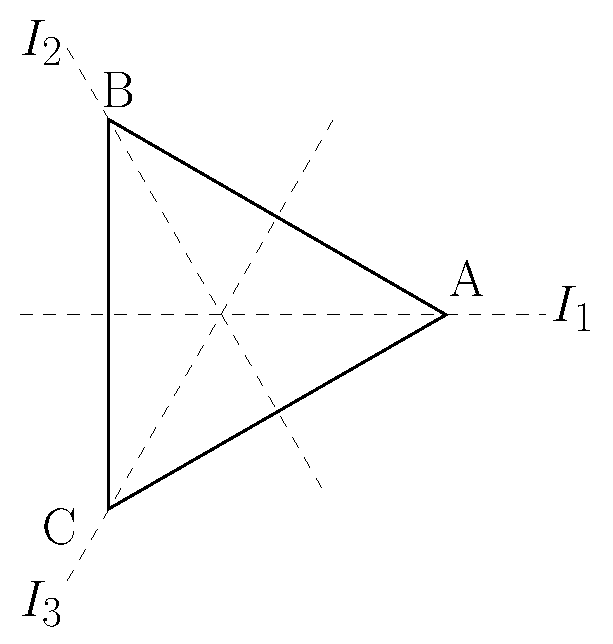
\includegraphics[width=.7\textwidth]{../../figs/D3triangle}
 		\end{center}
	$\Gamma x_A=\{x_B,x_C\}$
 	$\stab{x_A}=\{e,\Refl\}\cong\Dn{1}$
 	\end{exampleblock}
\end{columns}

\end{frame}

\frame{Fixed point subspaces}


\begin{frame}{Symmetry in differential equations}

\begin{block}{}
 We call a group element $\gamma\in\On{n}$ a symmetry of
\[
	\dot{x} = \vf(x,\lambda)\,,
	\label{eq:difeq} 
\]  
if for every solution $x(t)$, $\gamma x(t)$ is also a solution.
\end{block}

\end{frame}

\subsection{Desymmetrization of \CLe}

\begin{frame}{\CLe}
  \begin{columns}[t]
    \column{.4\textwidth}
    \begin{exampleblock}{\CLe}
      	\[
		\begin{split}
			\dot{x} &=-\sigma x+ \sigma y \,,\\
			\dot{y} &=(r-z)x-a y \,,\\
			\dot{z} &= \frac{1}{2}\left(x y^*+x^*y\right)-b z\,.
		\end{split}
	\]
    \end{exampleblock}
     \begin{block}{ }
       $x,y\in\Clx{}$, $z\in\Rls{}$ parameters $\sigma,\,b\in\Rls{}$, $r=r_1+i\, r_2$, $a=1-i\, e$, $r_1,\,r_2,\,e\in\Rls{}$.
    \end{block}

    \column{.5\textwidth}
    \begin{exampleblock}{Equivariant under}
	$SO(2)$ acting by
      	\[
	\begin{split}
 		\Rot{\theta} (x,y,z) &= (e^{i\theta} x, e^{i\theta} y, z)\,, \\
			\theta	& \in[0,2\pi)\,.
	\end{split}
	\]
    \end{exampleblock}
    \begin{exampleblock}{Physics}
	For $r_2=0$ appears as a truncation of Maxwell-Bloch equation
	that describes ring laser with detuning proportional to $e$.
    \end{exampleblock}

  \end{columns}
\end{frame}

\begin{frame}
  \begin{columns}[t]
     \column{.6\textwidth}
	\begin{block}{}
	\begin{center}
		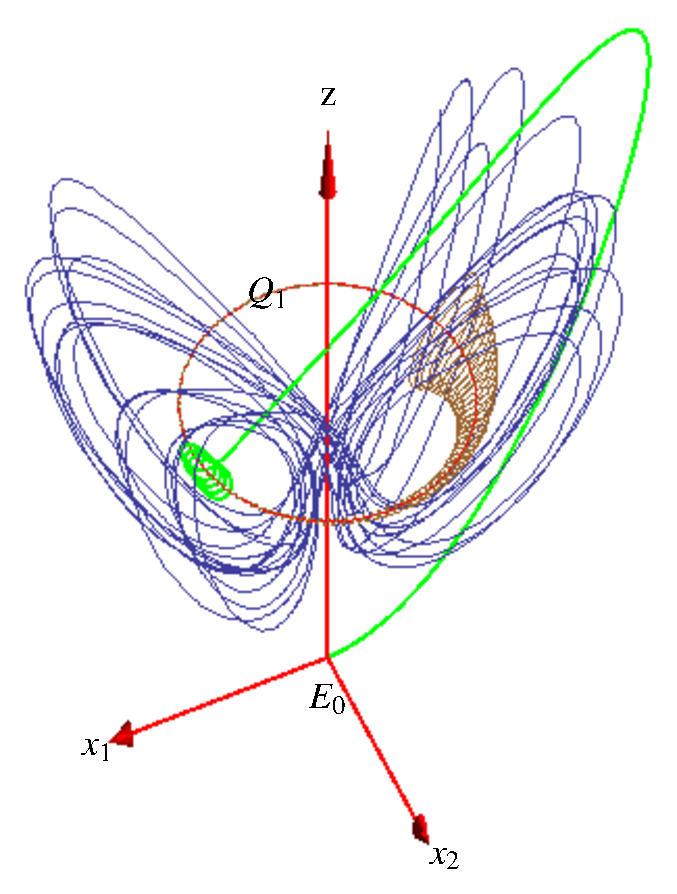
\includegraphics[width=.7\textwidth]{../../figs/CLE.eps}
	\end{center}
	\end{block}
     \column{.4\textwidth}
	\begin{block}{ }
	 ${r_1=28,}\, {b=8/3,}\,$ ${\sigma=10,}\, {a=1,}\,$ ${e=1/10,}\, {r_2=0}$
	\end{block}
	\begin{block}{ }
	  $E_0$: saddle\\
	  $Q_1$: relative equilibrium\\ 
	  $01$:  relative periodic orbit $T_{01}=1.542,\, \theta_{01}=2.953$
	\end{block}
   \end{columns}
\end{frame}

\begin{frame}{Symmetry reduction}
\begin{itemize}
 \item All points related by a symmetry operation (on the same group orbit) are mapped to the same point.
 \item Relative equilibria become equilibria and relative periodic orbits become periodic orbits in reduced space.
 \item Group orbits of equilibria or {\po s} are mapped to a single equilibrium or periodic orbit.
\end{itemize}
\end{frame}


\begin{frame}{\CLe\ reduction by invariant polynomials}

\begin{itemize}
 \item Usual approach: Rewrite the dynamics in a symmetry-invariant polynomial basis (Hilbert basis)
 \item For CLe it is (Gilmore and Letellier 2007):
		\[
		\begin{array}{ll}
			u_1 = x_1^2+x_2^2\,, &\qquad u_2 = y_1^2+y_2^2 \cont\,
			u_3 = x_1 y_2-x_2 y_1\,, &\qquad u_4 = x_1 y_1+x_2 y_2\cont\,
			u_5 = z\,,
% 			\label{eq:ipLaser}
		\end{array}
		\]
	where $x=x_1+i x_2$, $y=y_1+i y_2$.
 \item $u_i$'s are linearly independent but functionally related by the \emph{syzygy}
	\[
 		u_1 u_2 -u_3^2-u_4^2 =0\,.
	\]
 \item<alert@1-> Determination of Hilbert bases is computationally prohibitive as the dimension of the system increases (algebraic geometry algorithms)
 	\begin{itemize}
    	\item<alert@1-> In PDEs they have only been used for local problems (e.g. after center manifold reduction)
    	\end{itemize}
\end{itemize}

\end{frame}

\begin{frame}{\CLe\ reduction by invariant polynomials}

\begin{center}
%   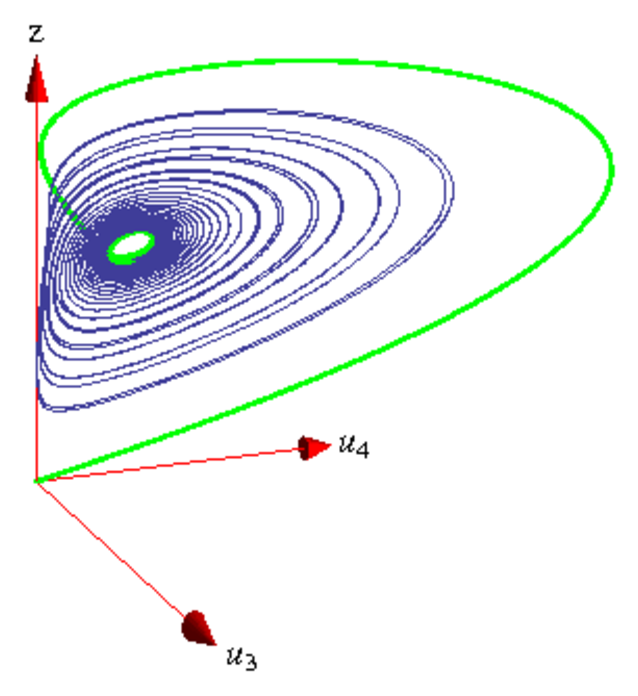
\includegraphics[width=0.35\textwidth]{../../figs/CLEip1}
  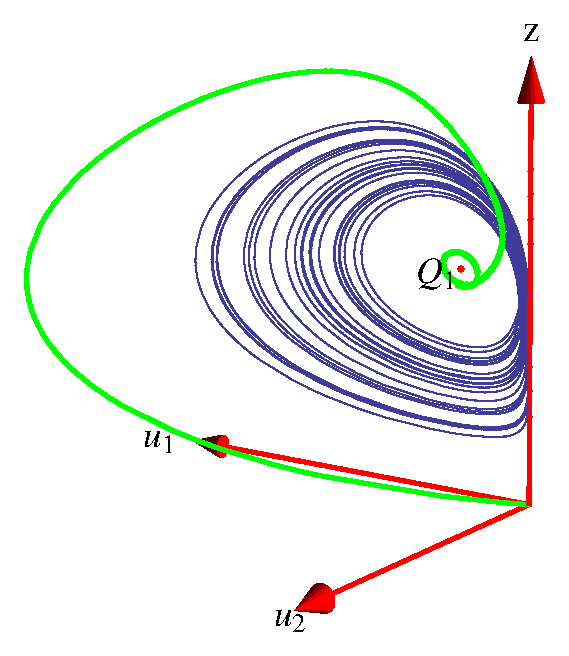
\includegraphics[width=0.36\textwidth]{../../figs/CLEip2} 
\end{center}

\end{frame}


\begin{frame}{Cross-sections and Moving frames}

\begin{block}{Moving frame}
 A smooth $\Gamma$-equivariant mapping $\rho:\,\Manif \rightarrow \Gamma$.
\end{block}

\begin{block}{Cross-section}
 An $(n-r)$-dimensional submanifold $K$ of $\Manif$ such that $K$ intersects each orbit transversally and at most once.
\end{block}

\begin{block}{}
Let $\Gamma$ act freely and regularly on M and let $K\subset\Manif$ be a cross-section.
For $x\in \Manif$, let $\gamma=\rho(x)$ be the unique group element that maps $x$ to the
cross-section: $\gamma x = \rho(x) x\, \in K$. Then $\rho:\Manif\rightarrow \Gamma$ is a right moving frame.
\end{block}

\end{frame}

\begin{frame}{Moving frame for \CLe.}

\begin{block}{Practical construction}
 \begin{itemize}
  \item Write out group transformations explicitly:
	\negvsp\[
		\begin{array}{ll}
		\overline{x}_1 = x_1 \cos\theta - x_2 \sin\theta\,, &
		\overline{x}_2 = x_1 \sin\theta + x_2 \cos\theta\cont
		\overline{y}_1 = y_1 \cos\theta - y_2 \sin\theta\,, &
		\overline{y}_2 = y_1 \sin\theta + y_2 \cos\theta\cont	
		\overline{z} = z\,.
		\end{array}
	\]
  \item \negvsp Define a cross-section $K_i(x)=c_i\,,\ i=1,\ldots r$:
	\negvsp\[
	 	K_i(x)=x_1=0\,.
	\]
  \item \negvsp Write the \emph{normalization equations} $K_i(\gamma x)=c_i\,,\ i=1,\ldots r$:
	\negvsp\[
		\gamma\, x_1=0\ \mathrm{or}\ \overline{x}_1=0.	 
	\]
  \item \negvsp Solve for the $r$ group parameters:
	\negvsp\[
	 	\theta=\tan^{-1}\frac{x_1}{x_2}
	\]

 \end{itemize}

\end{block}

\end{frame}

\begin{frame}{\CLe\ reduction}
 \begin{block}{Fundamental invariants}
	Substituting the expression for the moving frame back in the remaining group equations
	we get the \emph{fundamental invariants} for the problem:
  	\[
  	 \begin{split}
	\overline{x}_2 &= \sqrt{x_1^2+x_2^2} \cont
	\overline{y}_1 &= \frac{x_2 y_1-x_1 y_2}{\sqrt{x_1^2+x_2^2}}\cont
	\overline{y}_2 &=\frac{x_1 y_1+x_2 y_2}{\sqrt{x_1^2+x_2^2}}\,.
	\end{split}
  	\]
 \end{block}
\end{frame}


\begin{frame}{\CLe\ reduction II}
\end{frame}

\begin{frame}{\CLe\ reduction by double section}
\end{frame}


\section[\KSe]{\KS, $L=22$, phase space }

\subsection{\KSe}

\begin{frame}{\KSe}
\[
  u_t = F(u) = -{\textstyle\frac{1}{2}}(u^2)_x-u_{xx}-u_{xxxx}
    \,,\qquad   x \in [-L/2,L/2]
    \,,
\]
Appears in study of many extended systems including
\begin{itemize}
 \item reaction-diffusion systems
 \item combustion problems (flame fronts)
 \item thin falling films
 \item and more\ldots
\end{itemize}


Impose periodic boundary conditions:
\[
 u(x,t) = u(x+L,t)
\]
\end{frame}

\begin{frame}{Symmetries of \KSe}

\begin{itemize}
 \item Galilean invariance: if $u(x,t)$ is a solution, then $u(x-ct,t)-c$, with $c$ an arbitrary constant
	speed, is also a solution.
	\begin{itemize}
		\item The mean $u_0=\int_{-L/2}^{L/2} u dx$ is a constant of the motion. \\
		\item Setting $u_0=0$ corresponds to choosing $c=0$ therefore eliminating Galilean invariance.
	\end{itemize}
 \item Equivariant under $\On{2}$:
\[
	\Shift_{\shift/L}\, u(x,t) = u(x+\shift,t)\,,\qquad \shift\in\left[-L/2,L/2\right]\,,
\]

\[
    \Refl \, u(x) = -u(-x)
\,.
\]
\end{itemize}
\end{frame}

\begin{frame}{Fourier space}
Use
\[
  u(x,t)=\sum_{k=-\infty}^{+\infty} a_k (t) e^{ i q_k x }
\]
where
\[
 q_k = 2\pi\,k/L.
\]
Get
\[
 \dot{a}_k
     = ( q_k^2 - q_k^4 )\, a_k
    - i \frac{q_k}{2} \sum_{m=-\infty}^{+\infty} a_m a_{k-m}\,,
\]
with $a_{k}=a^\ast_{-k}$ since $u(x,t)$ is real.

Truncate to finite order $N$.
\end{frame}

\begin{frame}{Symmetry in Fourier space}

Symmetry acts as
\[
  \Shift_{\shift/L}\, a = \mathbf{g}(\shift) \, a \,,
  \label{eq:shiftF}
\]
\[
   \Refl \, a = -a^\ast
\]
where $\mathbf{g}(\shift) = \mathrm{diag}( e^{i q_k\, \shift} )$.

\end{frame}

\begin{frame}{Bifurcations}
\begin{center}
  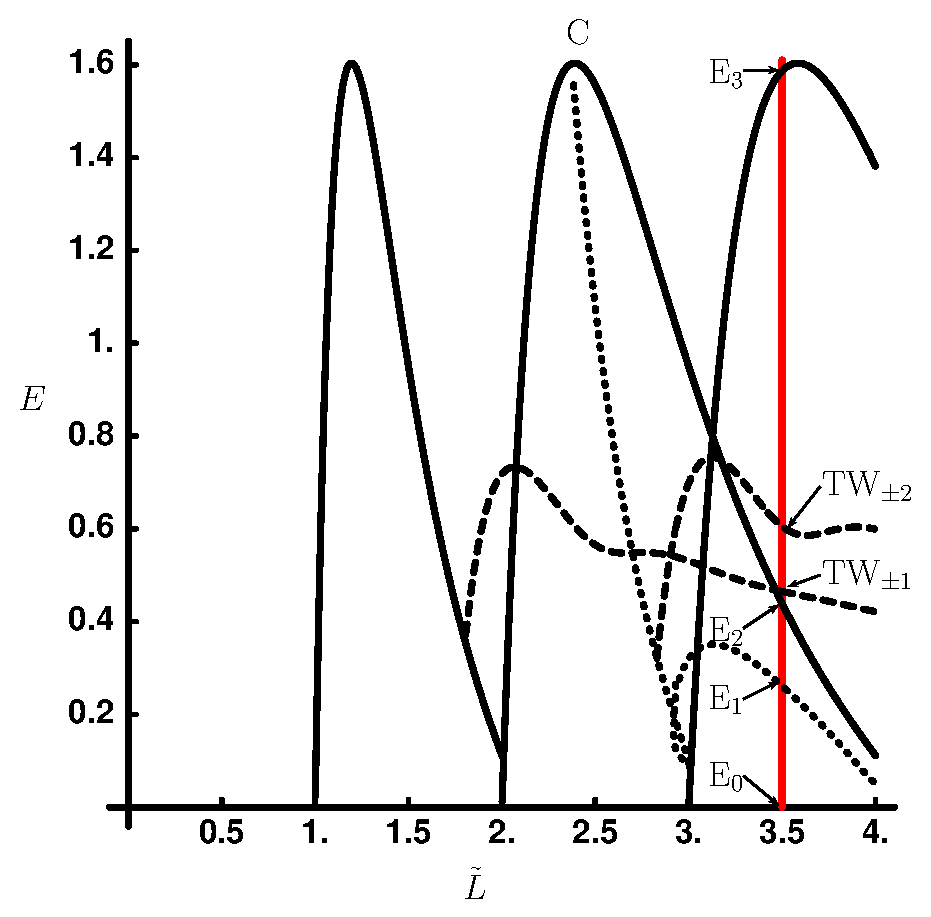
\includegraphics[width=0.5\textwidth]{../../figs/ksBifDiag}
\end{center}
\end{frame}


\begin{frame}{\eqva}
\begin{tabular}{ccc} ~~~\EQV{1} & ~~~\EQV{2} & ~~~\EQV{3} \vspace{12pt}\\
    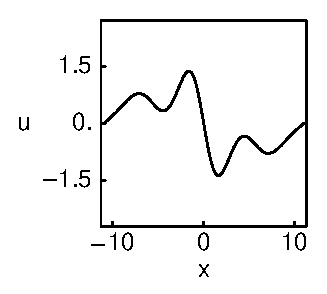
\includegraphics[width=0.25\textwidth]{../../figs/1wKS22equil}&
    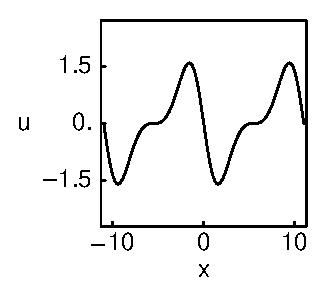
\includegraphics[width=0.25\textwidth]{../../figs/2wKS22equil}&
   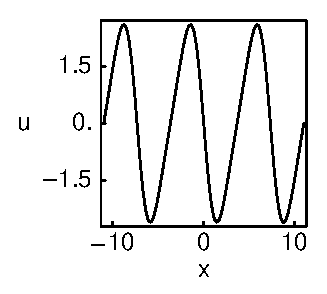
\includegraphics[width=0.25\textwidth]{../../figs/3wKS22equil}
\end{tabular}
\end{frame}

\begin{frame}{\reqva}
 \begin{tabular}{cc}
 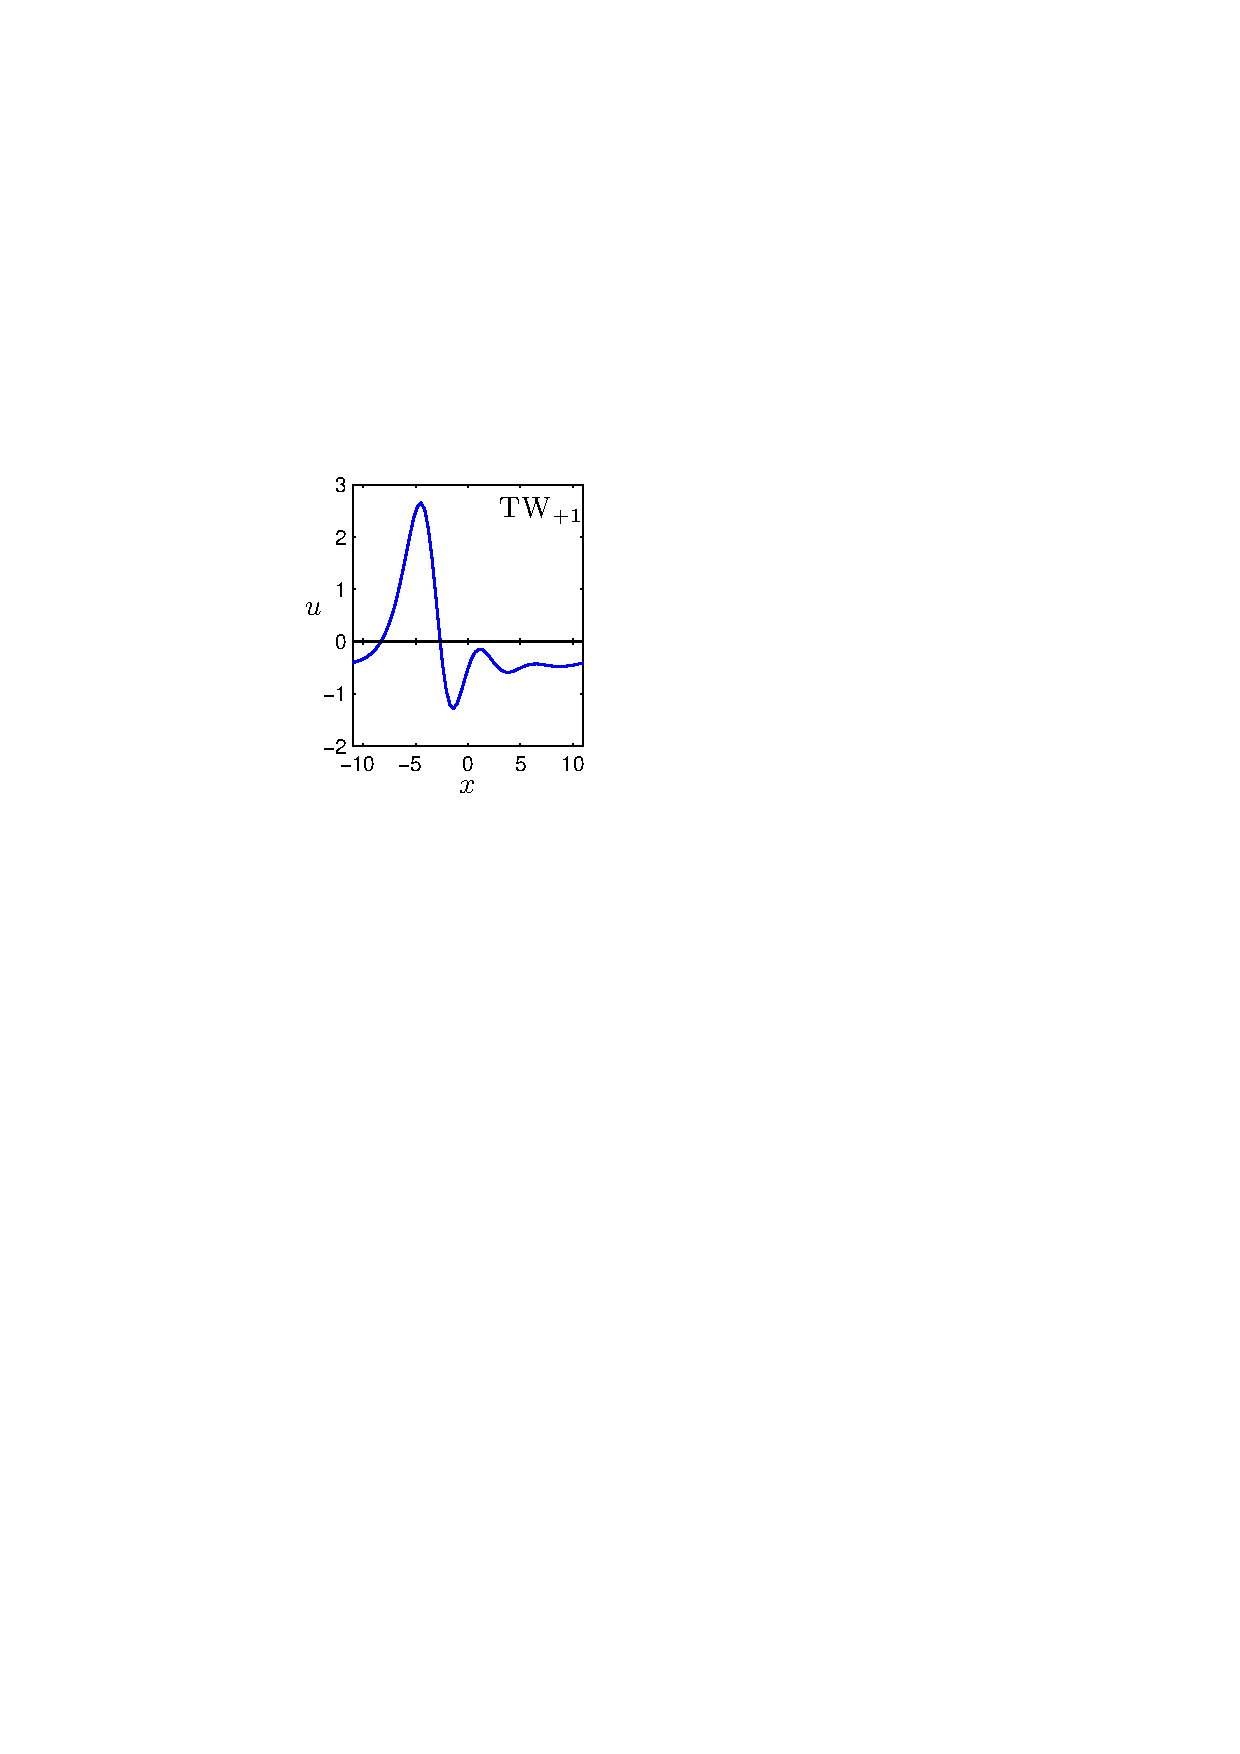
\includegraphics[width=0.25\textwidth]{../../figs/ks22_TW1_profile}
 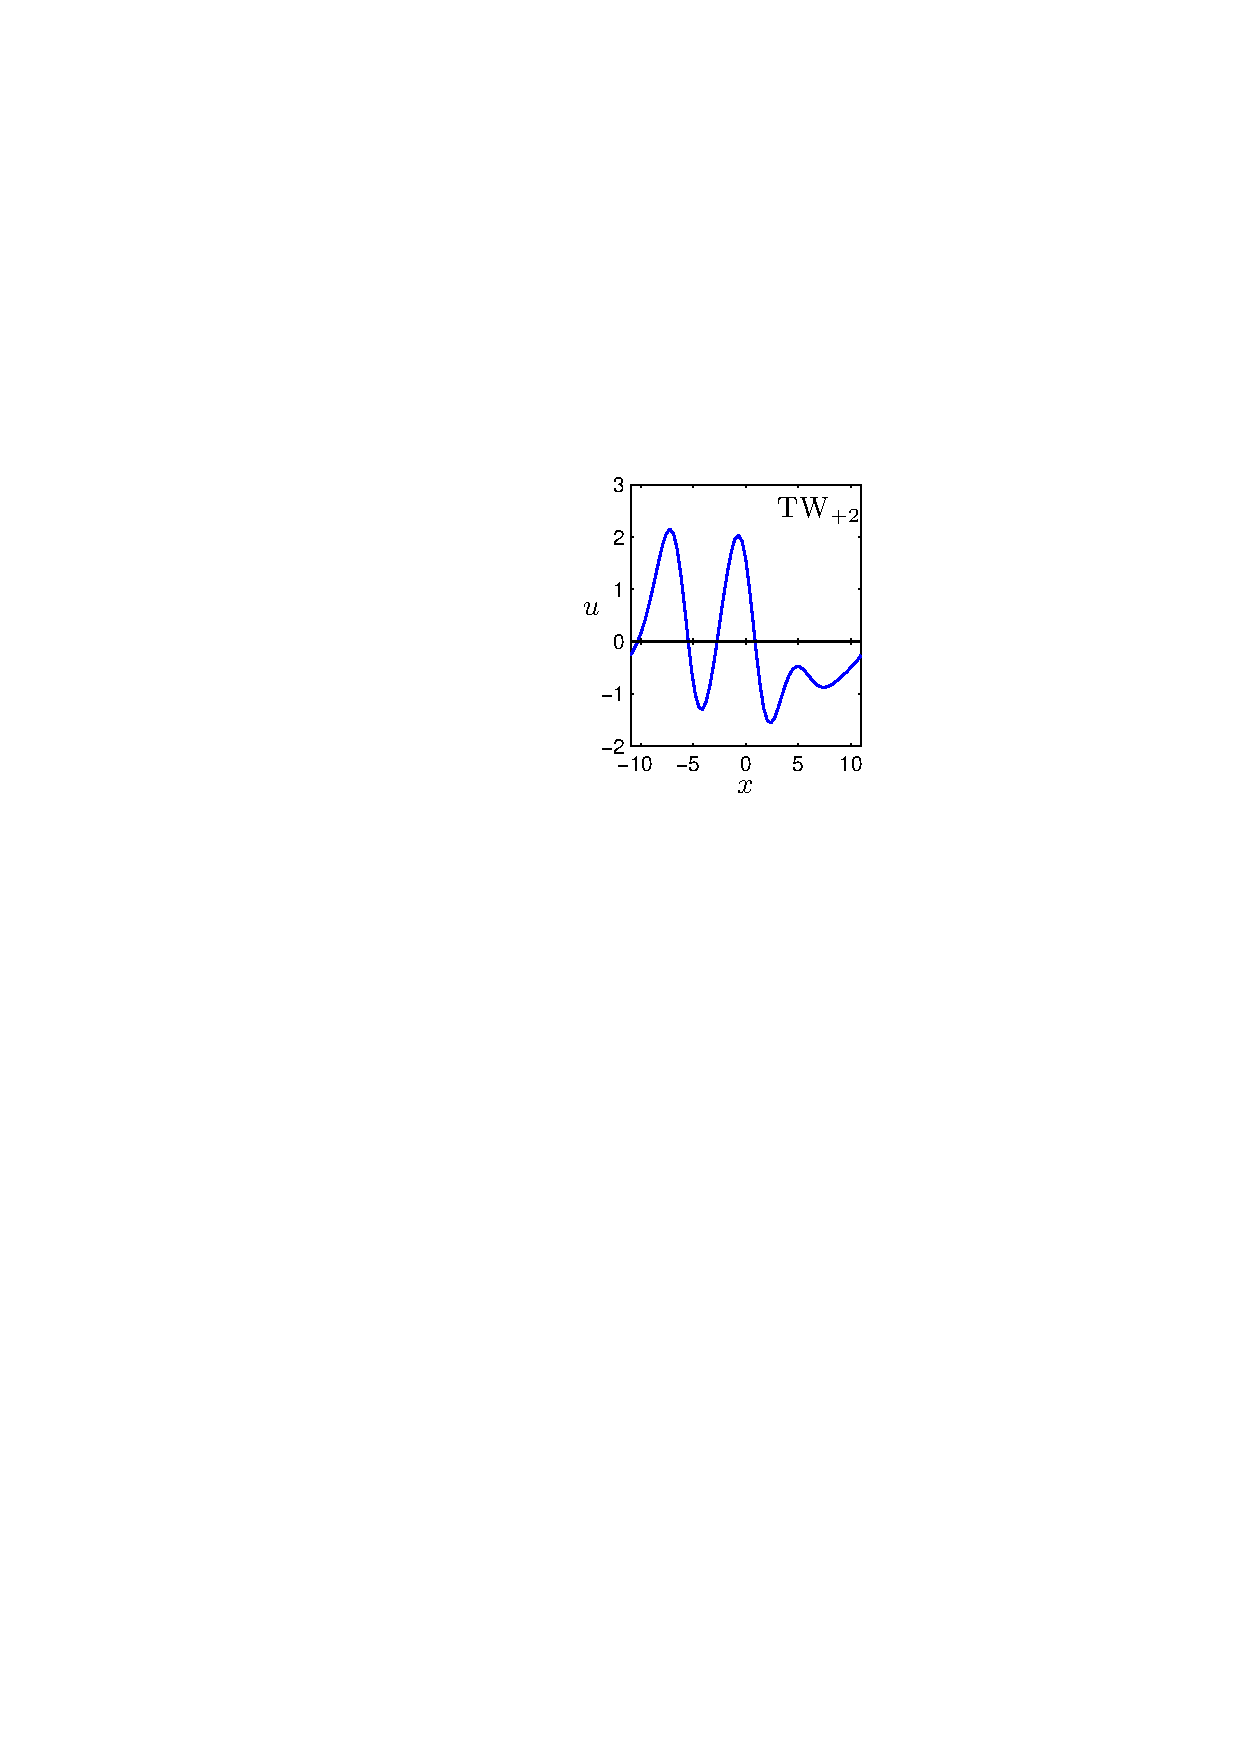
\includegraphics[width=0.25\textwidth]{../../figs/ks22_TW2_profile}\\
 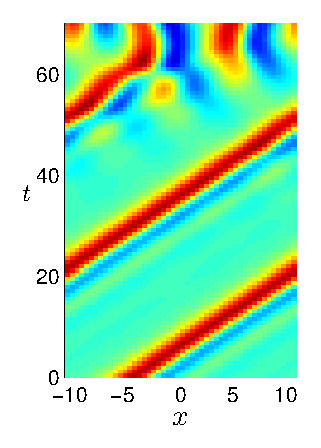
\includegraphics[width=0.25\textwidth]{../../figs/ks22_TW1_orbit_c}
 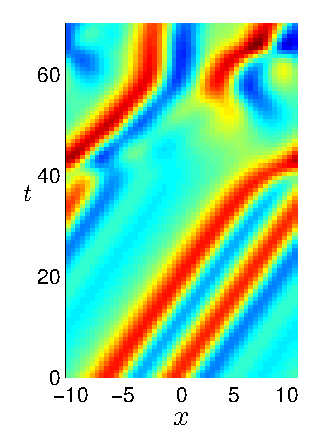
\includegraphics[width=0.25\textwidth]{../../figs/ks22_TW2_orbit_c}
 \end{tabular}
\end{frame}

\begin{frame}{Unstable manifolds: \EQV{1}}
 \begin{tabular}{cc}
 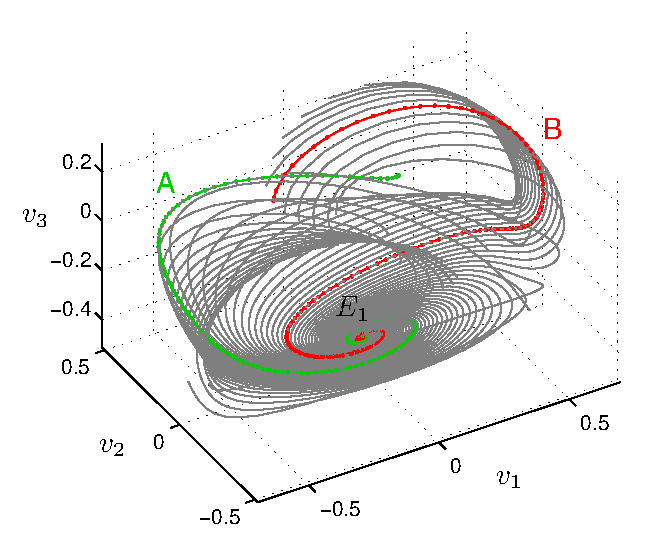
\includegraphics[width=0.3\textwidth]{../../figs/ks22_E1_plane1_manifold_c} &
 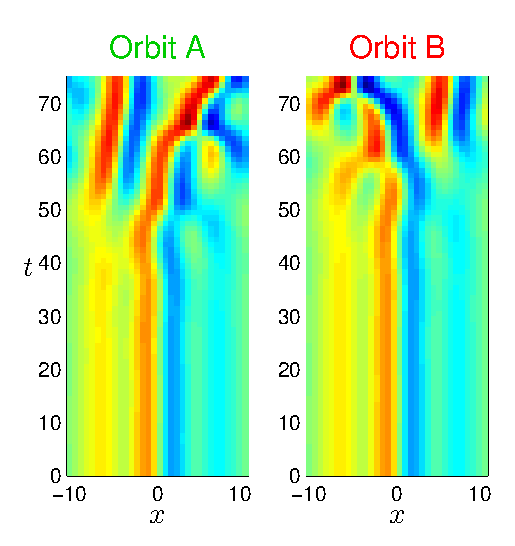
\includegraphics[width=0.2\textwidth]{../../figs/ks22_E1_plane1_orbits_c}\\
 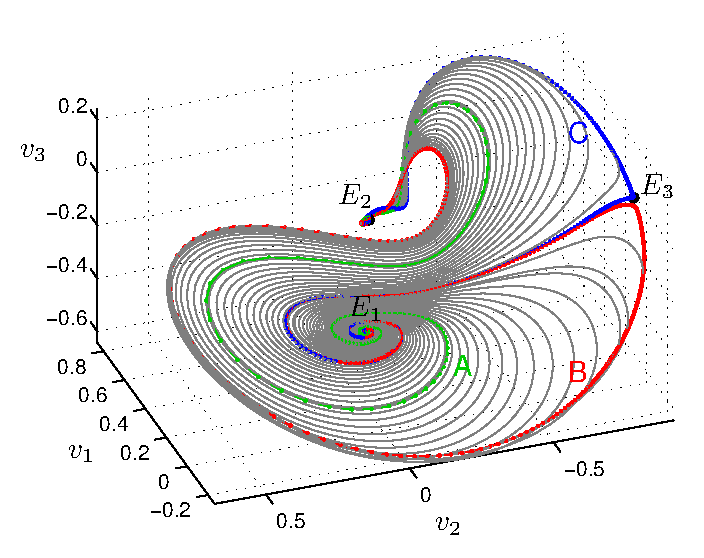
\includegraphics[width=0.3\textwidth]{../../figs/ks22_E1_plane2_manifold_c} &
 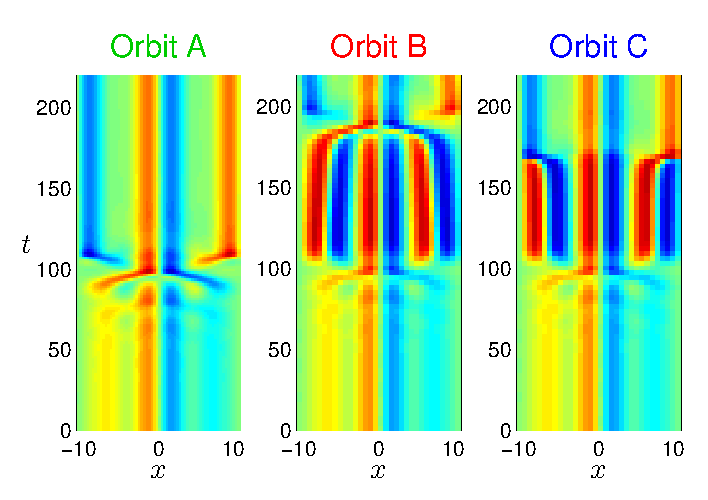
\includegraphics[width=0.32\textwidth]{../../figs/ks22_E1_plane2_orbits_c}
 \end{tabular}
\end{frame}

\begin{frame}{Unstable manifolds: \EQV{2}}
 \begin{tabular}{cc}
 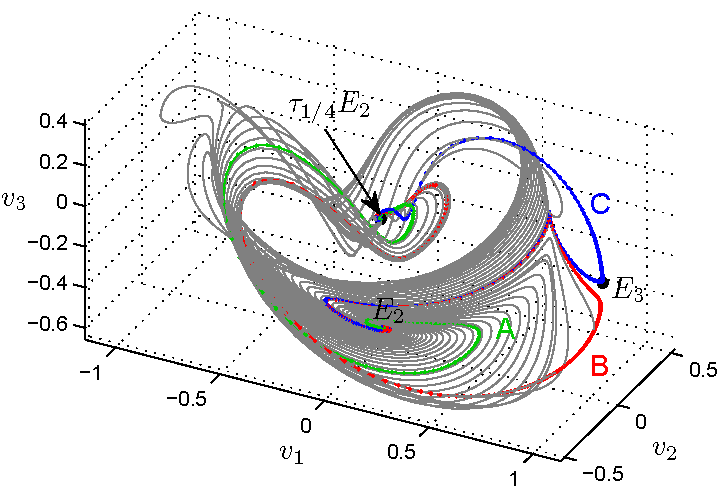
\includegraphics[width=0.48\textwidth]{../../figs/ks22_E2_manifold_c}
 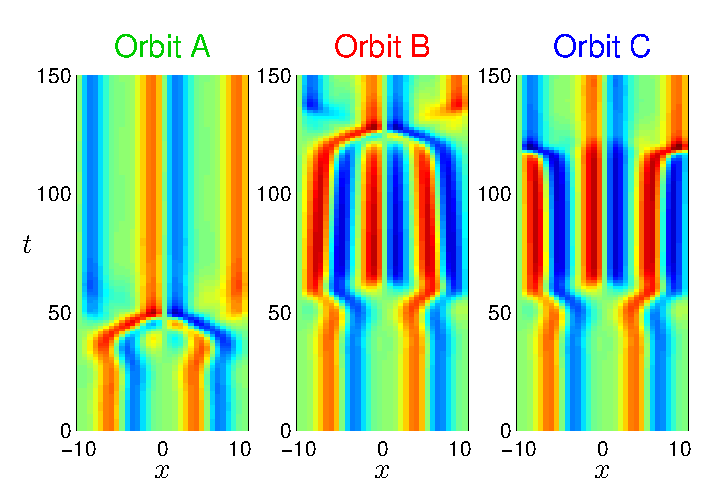
\includegraphics[width=0.48\textwidth]{../../figs/ks22_E2_orbits_c}
 \end{tabular}
\end{frame}

\begin{frame}{Unstable manifolds: \EQV{3}}
 \begin{tabular}{cc}
 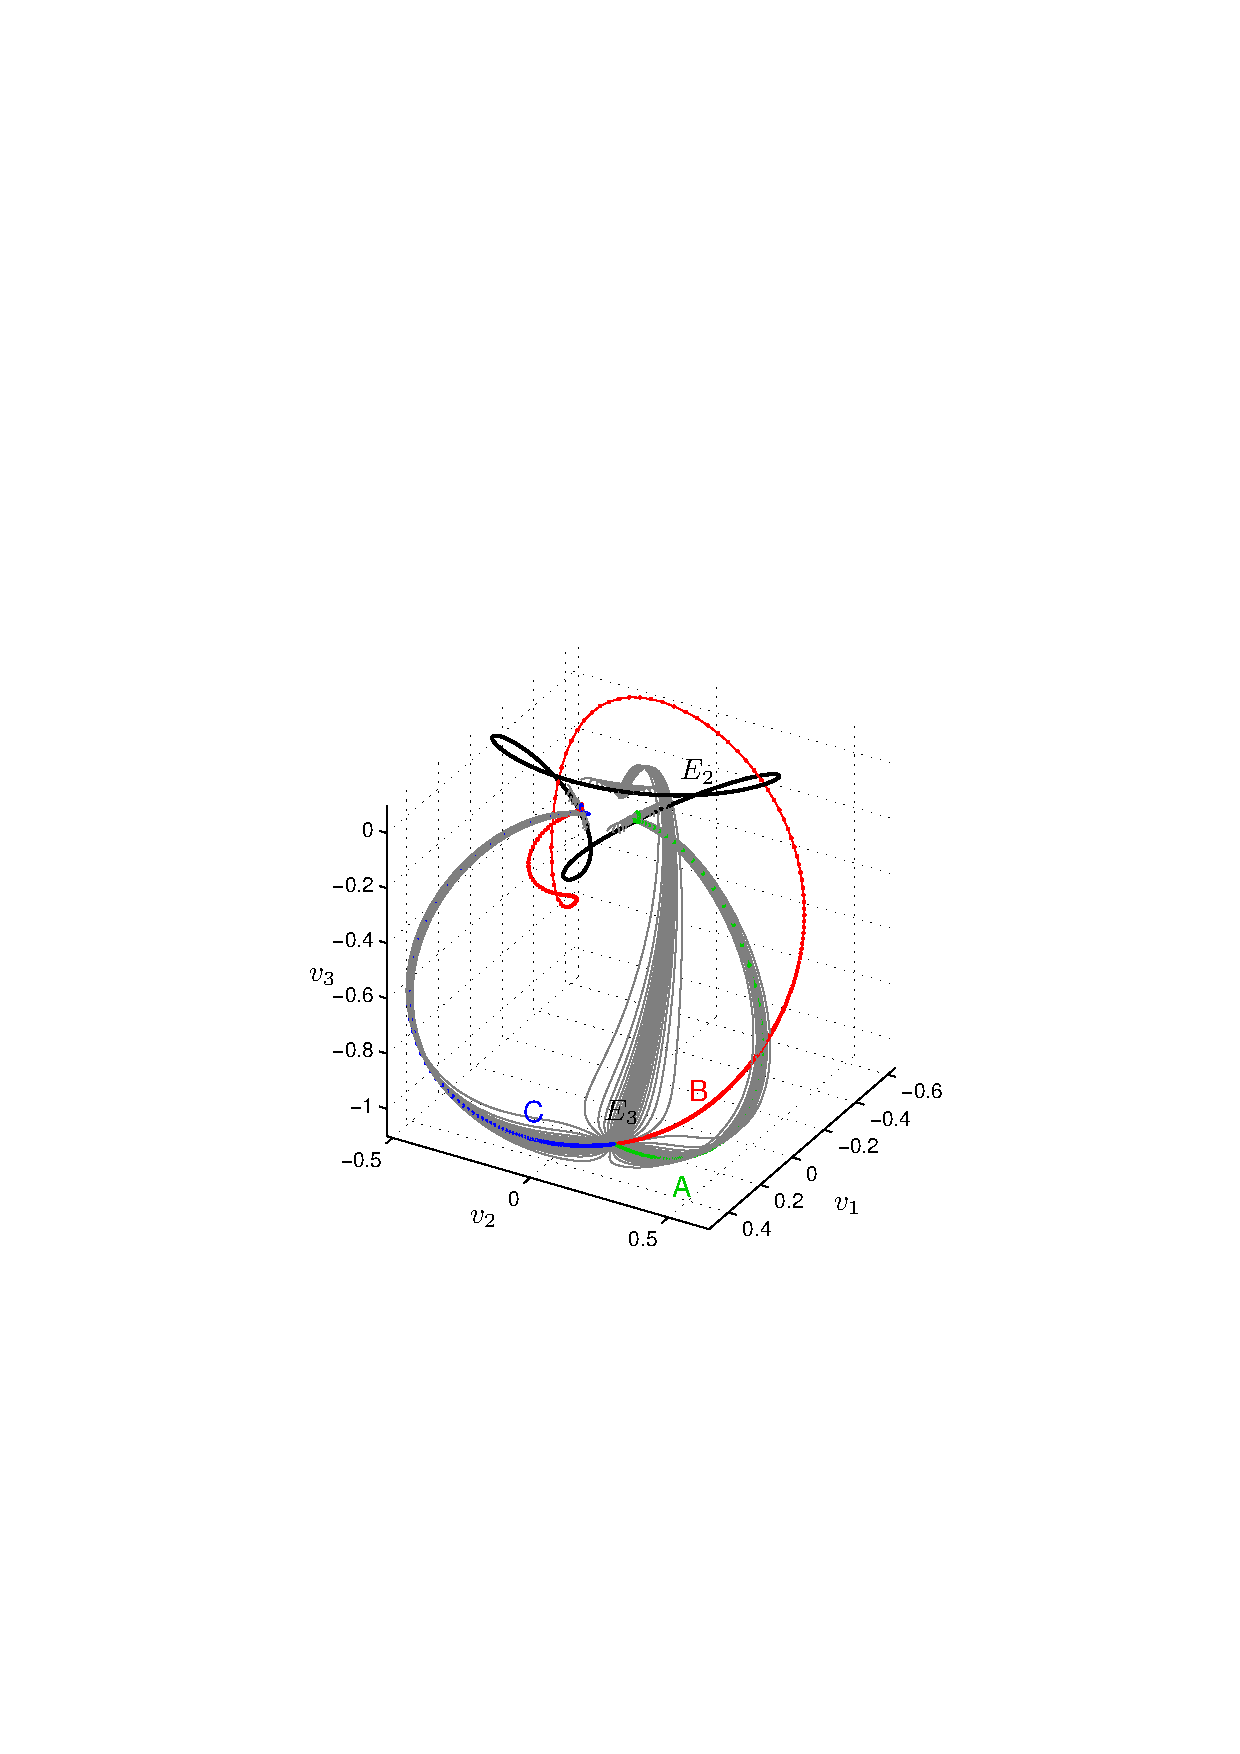
\includegraphics[width=0.45\textwidth]{../../figs/ks22_E3_manifold}
 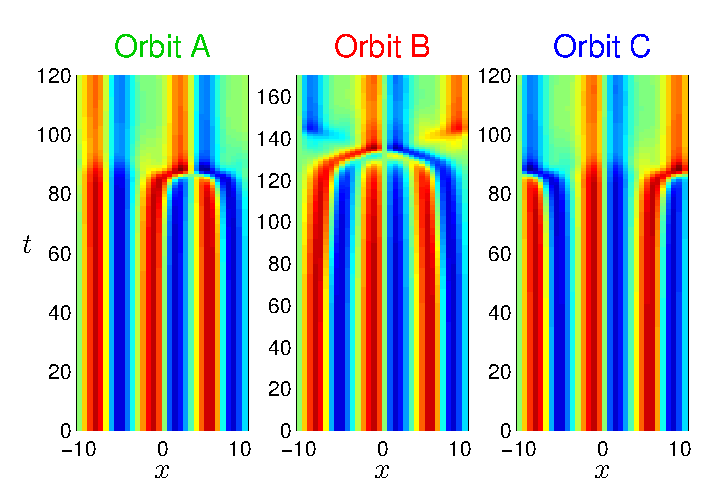
\includegraphics[width=0.5\textwidth]{../../figs/ks22_E3_orbits_c}	
 \end{tabular}
\end{frame}

\begin{frame}{Heteroclinic web}
         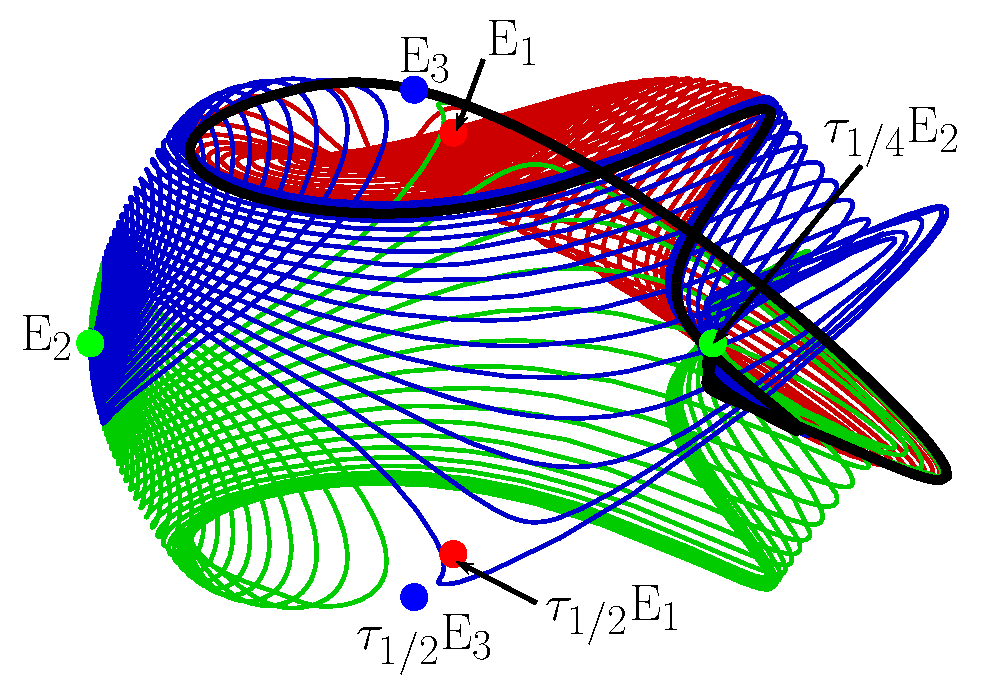
\includegraphics[width=0.6\textwidth]{../../figs/KS22hetero} 
\end{frame}

\begin{frame}{\Rpo s}


\scriptsize
 \begin{tabular}{cccccc} 
~~~$\period{p} = 16.3$, & ~~~$\period{p} = 33.5$,  & ~~~$\period{p} = 47.6$,  &
                         ~~~$\period{p} = 71.7$,  & ~~~$\period{p} = 10.3$ & ~~~$\period{p} = 33.4$\\
~~~$\shift_p = 2.86$ & ~~~$\shift_p = 4.04$ & ~~~$\shift_p = 5.68$ & ~~~$\shift_p = 5.503$ & &\\
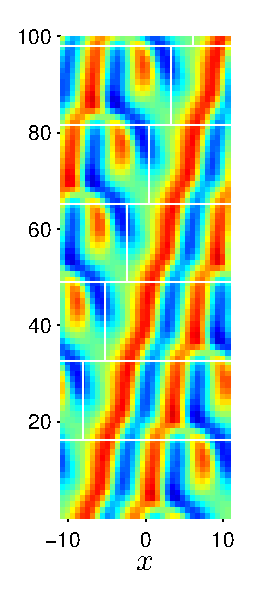
\includegraphics[width=0.15\textwidth]{../../figs/ks22rpo016.3-02.86.eps}\hspace{-3ex} &
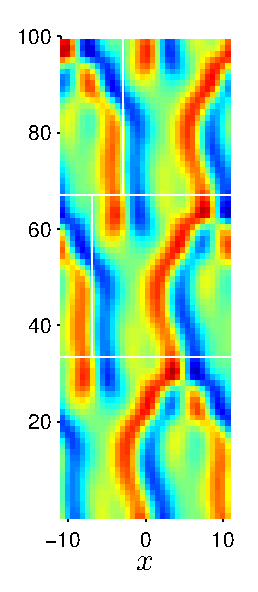
\includegraphics[width=0.15\textwidth]{../../figs/ks22rpo033.5-04.04.eps}\hspace{-3ex} &
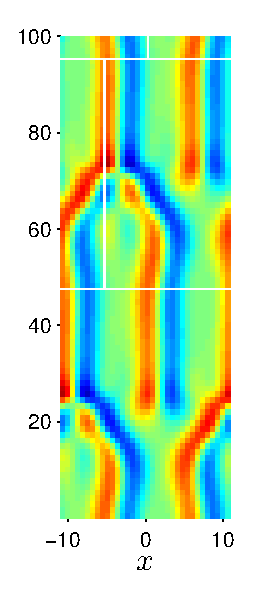
\includegraphics[width=0.15\textwidth]{../../figs/ks22rpo047.6-05.68.eps}\hspace{-3ex} &
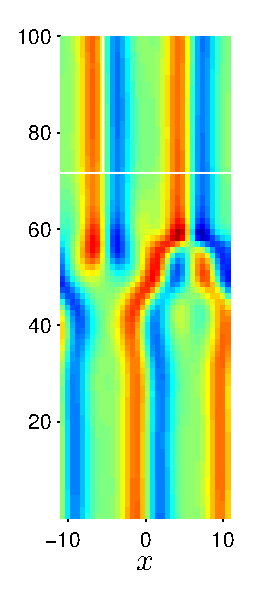
\includegraphics[width=0.15\textwidth]{../../figs/ks22rpo071.7-05.50.eps}\hspace{-3ex} &
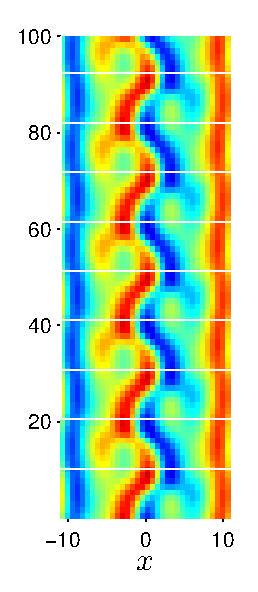
\includegraphics[width=0.15\textwidth]{../../figs/ks22rpo020.5-00.00.eps}\hspace{-3ex} &
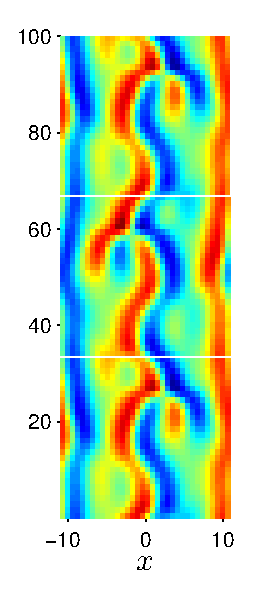
\includegraphics[width=0.15\textwidth]{../../figs/ks22rpo066.8-00.00.eps}\\
% $\period{p} = 32.8$, $\shift_p = 10.96$ & $\period{p} = 34.6$, $\shift_p = 9.60$ & $\period{p} = 59.9$, $\shift_p = 5.44$ &
% $\period{p} = 84.4$, $\shift_p = 5.513$ & $\period{p} = 32.4$ & $\period{p} = 35.2$\\
% 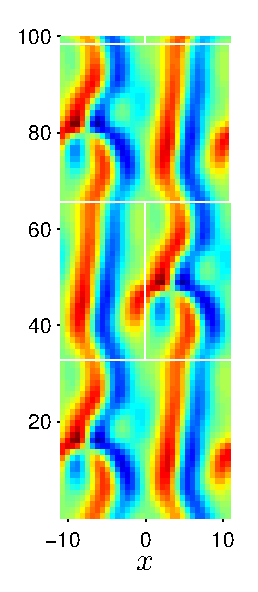
\includegraphics[width=0.15\textwidth]{../../figs/ks22rpo032.8-10.96.eps}\hspace{-3ex} &
% 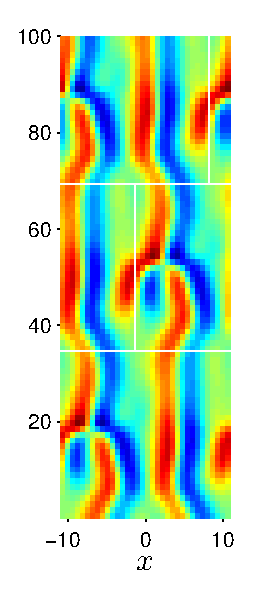
\includegraphics[width=0.15\textwidth]{../../figs/ks22rpo034.6-09.60.eps}\hspace{-3ex} &
% 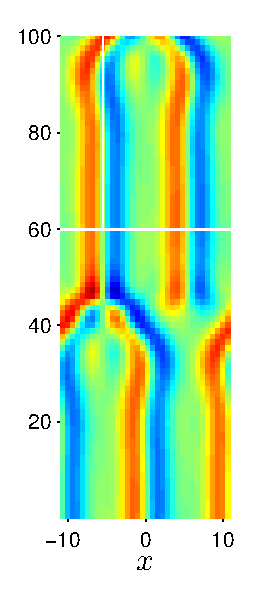
\includegraphics[width=0.15\textwidth]{../../figs/ks22rpo059.9-05.44.eps}\hspace{-3ex} &
% 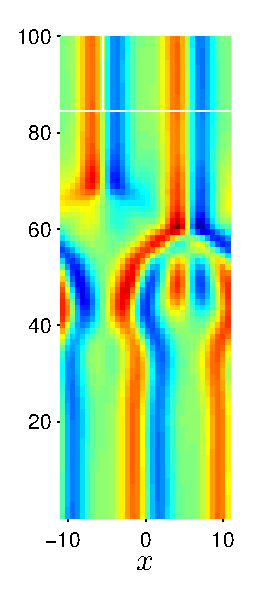
\includegraphics[width=0.15\textwidth]{../../figs/ks22rpo084.4-05.51.eps}\hspace{-3ex} &
% 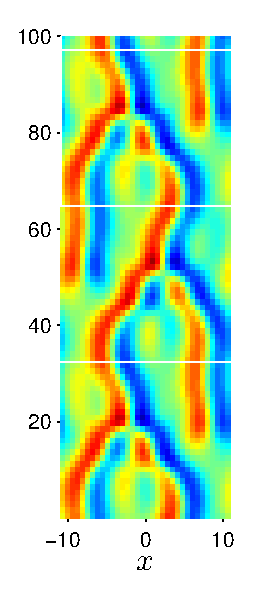
\includegraphics[width=0.15\textwidth]{../../figs/ks22rpo064.7-00.00.eps}\hspace{-3ex} &
% 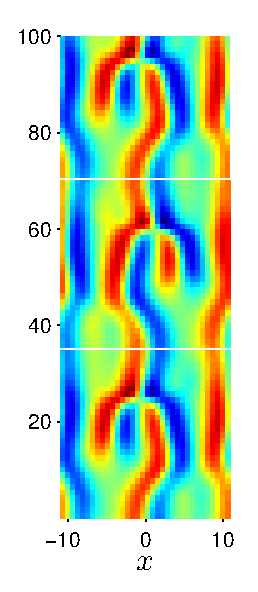
\includegraphics[width=0.15\textwidth]{../../figs/ks22rpo070.3-00.00.eps}
\end{tabular}
\end{frame}

\begin{frame}
 
\end{frame}




\subsection{Reduced space}

\section*{Summary}
\begin{frame}
\frametitle<presentation>{Summary}

In summary

\end{frame}


\end{document}
